\documentclass[12pt,a4paper]{article}

% Packages
\usepackage[utf8]{inputenc}
\usepackage[margin=1in]{geometry}
\usepackage{times}
\usepackage{graphicx}
\usepackage{hyperref}
\hypersetup{
    colorlinks=false,
    linkbordercolor=white,
    pdfborder={0 0 0}
}
\usepackage{setspace}
\usepackage{longtable}
\usepackage{array}
\usepackage{booktabs}
\usepackage{caption}
\usepackage{enumitem}
\usepackage{titlesec}

% Line spacing
\setstretch{1.15}

% Justify alignment
\setlength{\parindent}{0pt}
\setlength{\parskip}{3pt}

% Reduce excessive whitespace
\raggedbottom
\setlength{\topskip}{0pt}
\setlength{\floatsep}{10pt plus 2pt minus 2pt}
\setlength{\textfloatsep}{10pt plus 2pt minus 2pt}
\setlength{\intextsep}{10pt plus 2pt minus 2pt}

% Caption font
\captionsetup{font=footnotesize}

% Section formatting
\titleformat{\section}
  {\normalfont\fontsize{14}{16}\selectfont\bfseries\uppercase}{\thesection}{1em}{}
  
\titleformat{\subsection}
  {\normalfont\fontsize{12}{14}\selectfont\bfseries}{\thesubsection}{1em}{\underline}

\begin{document}

% IMPORTANT: Ensure upes_logo.png is in project root (or comment out line 38 if unavailable)

% Title Page
\begin{titlepage}
    \centering
    \vspace*{1cm}
    
    {\fontsize{18}{22}\selectfont \textbf{Software Requirements Specification}\par}
    \vspace{1.5cm}
    
    {\fontsize{16}{20}\selectfont \textbf{For}\par}
    \vspace{1.5cm}
    
    {\fontsize{16}{20}\selectfont \textbf{CampusCompute: A Private Academic Cloud for Utilizing Idle Laboratory Resources}\par}
    \vspace{1cm}
    
    {\fontsize{14}{18}\selectfont October 2026\par}
    \vspace{2cm}
    
    {\fontsize{12}{16}\selectfont \textbf{Prepared by}\par}
    \vspace{0.5cm}
    
    \begin{table}[h]
    \centering
    \fontsize{10}{12}\selectfont
    \begin{tabular}{|l|l|l|l|}
    \hline
    \textbf{S.No} & \textbf{Specialization} & \textbf{SAP ID} & \textbf{Name} \\
    \hline
    1 & FullStack AI B-1 & 500120595 & Kuldeep Chaudhary \\
    \hline
    2 & CCVT B-1 & 500119484 & Rishu Raj \\
    \hline
    3 & CCVT B-2 & 500125960 & Daksh Mehrotra \\
    \hline
    4 & CCVT B-5 & 500122440 & Krishna Bisht \\
    \hline
    \end{tabular}
    \end{table}
    
    \vspace{1cm}
    {\fontsize{12}{16}\selectfont \textbf{Project Mentor: Dr. Mohd Hanief Wani}\par}
    \vspace{2cm}
    
    
\includegraphics[width=0.3\textwidth]{upes_logo.png}
    
    \vspace{0.5cm}
    {\fontsize{12}{16}\selectfont
    Department of Informatics\\
    School of Computer Science\\
    UNIVERSITY OF PETROLEUM \& ENERGY STUDIES,\\
    DEHRADUN- 248007, Uttarakhand\par}
\end{titlepage}

\newpage

% Table of Contents
\tableofcontents
\newpage

% Revision History
\section*{Revision History}
\addcontentsline{toc}{section}{Revision History}

\begin{table}[h]
\fontsize{10}{12}\selectfont
\begin{tabular}{|p{3cm}|p{4cm}|p{5cm}|p{3cm}|}
\hline
\textbf{Date} & \textbf{Change} & \textbf{Reason for Changes} & \textbf{Mentor Signature} \\
\hline
August 15, 2026 & Initial draft & Project scope definition and requirement gathering & \\
\hline
September 5, 2026 & Added system architecture & Technical design and component specification & \\
\hline
September 18, 2026 & Updated diagrams & Added all UML diagrams per template requirements & \\
\hline
September 28, 2026 & Document finalization & Final version after mentor feedback and corrections & \\
\hline
\end{tabular}
\end{table}

\newpage

% 1. INTRODUCTION
\section{INTRODUCTION}

\subsection{Purpose of the Project}

CampusCompute addresses underutilized computing resources in educational institutions (60-70\% idle time) while providing students free access to high-performance infrastructure. Most college labs remain idle during non-operating hours, weekends, and holidays despite significant capital investment (Rs. 1-5 Crore). Meanwhile, students face prohibitive cloud service costs (Rs. 2000-5000/month).

CampusCompute transforms idle lab computers into a private cloud, enabling on-demand isolated containerized environments accessible 24/7 from anywhere. At UPES, 250 lab computers (Rs. 1.25 Crore) with 1500 CPU cores operate at only 20\% utilization. CampusCompute increases this to 60-70\%, multiplying institutional computing capacity without additional hardware.

\subsection{Target Beneficiary}

\textbf{Students:} CS/Data Science/AI-ML students needing high-performance computing for projects; economically disadvantaged students unable to afford expensive hardware or cloud subscriptions; remote learners requiring lab access outside campus hours.

\textbf{Educational Institutions:} IT departments maximizing ROI on lab infrastructure; lab administrators managing 100-500 computers; academic departments with cloud budget constraints.

\textbf{Faculty:} Course instructors assigning computationally intensive projects; researchers needing distributed computing; lab coordinators monitoring resource usage.

\subsection{Project Scope}

CampusCompute applies to educational institutions with existing lab infrastructure, enabling resource pooling, on-demand container provisioning, and secure multi-tenant access.

\textbf{Benefits:} Eliminate Rs. 5-10 lakhs annual cloud costs; increase utilization from 20\% to 60-70\%; 24/7 remote access; support 500+ devices and 2000+ containers; isolated secure environments.

\textbf{Objectives:}
\begin{enumerate}[noitemsep]
    \item Deploy distributed container orchestration across campus labs
    \item Implement intelligent scheduling for optimal resource allocation
    \item Provide web interface for container management and terminal access
    \item Establish secure WebSocket communication between backend and agents
    \item Support multi-organization architecture with quota management
\end{enumerate}

\textbf{Goals:} Container creation in 5-10 seconds; support 100+ concurrent devices with 500+ containers; 99\%+ uptime; reduce student cloud expenses by 90-95\%; one-click agent deployment.

\textbf{Deliverables:} Backend (Spring Boot with REST/WebSocket), Frontend (React portal), Python agent, Windows installer, PostgreSQL schema, documentation (installation, API, user manuals), architecture diagrams.

\subsection{References}

\begin{enumerate}[noitemsep]
    \item Docker Documentation - Container Platform Architecture. \textit{https://docs.docker.com/}
    \item Spring Boot Framework Documentation. \textit{https://spring.io/projects/spring-boot}
    \item WebSocket Protocol (RFC 6455). \textit{https://datatracker.ietf.org/doc/html/rfc6455}
    \item PostgreSQL Database Documentation. \textit{https://www.postgresql.org/docs/}
    \item React Frontend Framework. \textit{https://react.dev/}
    \item xterm.js - Terminal Emulator for Web. \textit{https://xtermjs.org/}
    \item IEEE Standard for Software Requirements Specifications (IEEE 830-1998)
    \item Project Documentation: PROJECT\_DOCUMENTATION.md (Internal)
\end{enumerate}

% 2. PROJECT DESCRIPTION
\section{PROJECT DESCRIPTION}

\subsection{Reference Algorithm}

\textbf{Primary Algorithm: Adaptive Device Scoring and Selection}

CampusCompute implements a multi-factor scoring algorithm for intelligent device selection when allocating containers. This algorithm ensures optimal resource distribution, load balancing, and high availability.

\textbf{Algorithm Steps:}

\begin{verbatim}
Function: selectBestDevice(requestedCPU, requestedRAM, requestedDisk)
Input: Container resource requirements
Output: Selected Device ID

1. Fetch all ONLINE devices from database
2. For each device:
   a. Calculate availableResources:
      - availableCPU = totalCPU - allocatedCPU
      - availableRAM = totalRAM - allocatedRAM
      - availableDisk = totalDisk - allocatedDisk
   
   b. Check if device can fulfill request:
      IF (availableCPU >= requestedCPU AND 
          availableRAM >= requestedRAM AND 
          availableDisk >= requestedDisk)
      THEN device is candidate
      ELSE skip device
   
   c. Calculate device score (0-100):
      score = (w1 * cpuScore) + (w2 * ramScore) + 
              (w3 * diskScore) + (w4 * containerScore) + 
              (w5 * healthScore)
   
   Where:
   - cpuScore = (availableCPU / totalCPU) * 100
   - ramScore = (availableRAM / totalRAM) * 100
   - diskScore = (availableDisk / totalDisk) * 100
   - containerScore = (1 - activeContainers/maxContainers) * 100
   - healthScore = deviceHealthStatus (100=healthy, 50=warning, 0=error)
   
   Weights (configurable):
   - w1 = 0.30 (CPU weight)
   - w2 = 0.30 (RAM weight)
   - w3 = 0.15 (Disk weight)
   - w4 = 0.15 (Container count weight)
   - w5 = 0.10 (Health weight)
   
3. Sort candidates by score (descending)
4. Return device with highest score
5. If no candidate found, throw NoDeviceAvailableException
\end{verbatim}

\textbf{Example Calculation:}

Device Specs: 8 CPU cores, 16GB RAM, 500GB disk, 3 active containers\\
Request: 2 CPU, 4GB RAM, 50GB disk

\begin{verbatim}
Available: 6 CPU, 12GB RAM, 450GB disk

cpuScore = (6/8) * 100 = 75.0
ramScore = (12/16) * 100 = 75.0
diskScore = (450/500) * 100 = 90.0
containerScore = (1 - 3/10) * 100 = 70.0
healthScore = 100 (healthy device)

Final Score = (0.30*75) + (0.30*75) + (0.15*90) + (0.15*70) + (0.10*100)
            = 22.5 + 22.5 + 13.5 + 10.5 + 10
            = 79.0
\end{verbatim}

\textbf{Data Structures Used:}

\begin{enumerate}[noitemsep]
    \item \textbf{Priority Queue/List:} For sorting devices by computed scores
    \item \textbf{Hash Map:} For storing device metrics (deviceId to metrics)
    \item \textbf{Database Indices:} B-tree indices on device status, organization\_id for fast queries
    \item \textbf{WebSocket Connection Pool:} HashMap mapping deviceId to WebSocket session
    \item \textbf{Container State Machine:} Finite State Automaton (FSA) managing lifecycle transitions
\end{enumerate}

\subsection{Characteristic of Data}

\textbf{Primary Data Sources:}

\begin{enumerate}[noitemsep]
    \item \textbf{System Metrics (Real-time):}
    \begin{itemize}[noitemsep]
        \item Source: Agent monitoring (psutil library)
        \item Frequency: Every 60 seconds
        \item Metrics: CPU usage (\%), RAM usage (bytes), disk usage (bytes), network I/O
        \item Processing: Time-series aggregation, moving averages
    \end{itemize}
    
    \item \textbf{Container Metadata:}
    \begin{itemize}[noitemsep]
        \item Source: Docker Engine API via docker-py
        \item Data: Container ID, status, image, ports, resource limits, creation timestamp
        \item Storage: PostgreSQL relational database
    \end{itemize}
    
    \item \textbf{User Activity Logs:}
    \begin{itemize}[noitemsep]
        \item Source: Backend application logs
        \item Data: User actions, API calls, authentication events, container operations
        \item Storage: Structured logs (JSON format)
        \item Processing: Log aggregation for analytics
    \end{itemize}
    
    \item \textbf{Device Inventory:}
    \begin{itemize}[noitemsep]
        \item Source: Agent enrollment process
        \item Data: Hostname, CPU specs, RAM capacity, disk space, operating system
        \item Collection Method: One-time during installation, updated on reconnection
    \end{itemize}
\end{enumerate}

\textbf{Secondary Data Sources:}

\begin{enumerate}[noitemsep]
    \item Docker Hub public images metadata
    \item Configuration files (YAML format)
    \item Enrollment tokens database
\end{enumerate}

\textbf{Data Processing Methods:}

\begin{itemize}[noitemsep]
    \item \textbf{Normalization:} Resource metrics normalized to 0-100 scale for scoring
    \item \textbf{Aggregation:} Real-time metrics aggregated per device and organization
    \item \textbf{Filtering:} SQL queries with WHERE clauses filtering by status, organization
    \item \textbf{Validation:} Input validation using Bean Validation (JSR-380)
\end{itemize}

\subsection{SWOT Analysis}

\begin{table}[h]
\fontsize{10}{12}\selectfont
\begin{tabular}{|p{7.5cm}|p{7.5cm}|}
\hline
\textbf{Strengths} & \textbf{Weaknesses} \\
\hline
\begin{itemize}[noitemsep,leftmargin=*]
    \item Zero cost for students (free cloud alternative)
    \item Utilizes existing infrastructure (no new hardware)
    \item 93\% cost savings vs AWS/Azure
    \item On-premise data (privacy \& compliance)
    \item Low latency (<10ms LAN vs 50-200ms WAN)
    \item Simple user experience (1-click container creation)
    \item Multi-organization support (scalable architecture)
\end{itemize} &
\begin{itemize}[noitemsep,leftmargin=*]
    \item Limited to campus lab capacity
    \item Requires Docker on each agent machine
    \item Network dependency (WebSocket connectivity)
    \item Windows-centric installer (Linux manual setup)
    \item Initial setup complexity for IT administrators
    \item Not suitable for GPU-intensive workloads (current version)
\end{itemize} \\
\hline
\textbf{Opportunities} & \textbf{Threats} \\
\hline
\begin{itemize}[noitemsep,leftmargin=*]
    \item Expand to 500+ institutions nationwide
    \item Add GPU support for AI/ML workloads
    \item Integration with LMS (Moodle, Canvas)
    \item Marketplace for container images
    \item Federation (share resources between universities)
    \item White-label SaaS offering
    \item Government grants for educational technology
\end{itemize} &
\begin{itemize}[noitemsep,leftmargin=*]
    \item Cloud providers offering student credits (AWS Educate)
    \item Security vulnerabilities in container escape
    \item Resistance from IT departments (change management)
    \item Docker licensing changes
    \item Network firewall restrictions
    \item Competing open-source solutions (OpenStack)
\end{itemize} \\
\hline
\end{tabular}
\caption{SWOT Analysis of CampusCompute}
\end{table}

\subsection{Project Features}

\textbf{Major Features:}

\begin{enumerate}[noitemsep]
    \item \textbf{Container Lifecycle Management}
    \begin{itemize}[noitemsep]
        \item Create containers with custom CPU, RAM, disk allocations
        \item AWS-style state transitions (PENDING to CREATING to RUNNING to STOPPING to STOPPED to RESTARTING to DELETED)
        \item Real-time status updates via WebSocket
        \item Automatic container expiration and cleanup
        \item Support for multiple Docker images (Ubuntu, Alpine, Python, Node.js)
    \end{itemize}
    
    \item \textbf{Intelligent Resource Scheduling}
    \begin{itemize}[noitemsep]
        \item Multi-factor device scoring algorithm
        \item Load balancing across devices
        \item Quota enforcement per user and organization
        \item Resource limit validation before allocation
        \item Priority-based scheduling (future enhancement)
    \end{itemize}
    
    \item \textbf{Web-Based Terminal Access}
    \begin{itemize}[noitemsep]
        \item Browser-based terminal using xterm.js
        \item WebSocket-based real-time communication
        \item Full shell access to containers
        \item Support for command history, scrollback buffer
        \item Secure authenticated sessions
    \end{itemize}
    
    \item \textbf{Multi-Tenancy and Role-Based Access Control}
    \begin{itemize}[noitemsep]
        \item Organization-level isolation
        \item Three roles: STUDENT, FACULTY, ADMIN
        \item JWT-based authentication
        \item Resource quotas per organization
        \item Lab-level access control
    \end{itemize}
    
    \item \textbf{Real-Time Monitoring and Analytics}
    \begin{itemize}[noitemsep]
        \item Device health monitoring (CPU, RAM, disk, network)
        \item Container metrics collection
        \item Heartbeat mechanism (30-second intervals)
        \item Automatic device offline detection
        \item Admin dashboard with live statistics
    \end{itemize}
    
    \item \textbf{One-Click Agent Deployment}
    \begin{itemize}[noitemsep]
        \item Windows GUI installer
        \item Automatic Docker Desktop installation
        \item Automatic Python environment setup
        \item Windows service registration
        \item Enrollment token-based authentication
        \item Progress tracking with detailed logging
    \end{itemize}
    
    \item \textbf{Device and Lab Management}
    \begin{itemize}[noitemsep]
        \item Register and manage multiple labs
        \item Generate enrollment tokens for device onboarding
        \item View device status, specifications, container counts
        \item Update device metadata
        \item Remove/decommission devices
    \end{itemize}
    
    \item \textbf{User Management}
    \begin{itemize}[noitemsep]
        \item Bulk student registration via CSV upload
        \item User creation with roles and quotas
        \item Password reset and first-time login flow
        \item User activity tracking
        \item Organization-specific user isolation
    \end{itemize}
\end{enumerate}

\subsection{User Classes and Characteristics}

\textbf{User Class 1: Student}

\textit{Characteristics:} Primary users (80-90\%); basic to intermediate proficiency; age 18-25; access 3-5 times/week for 1-4 hours.

\textit{Use Cases:} Login, create containers with specific resources, access web terminal, run code/compile programs, stop/restart containers, view container list.

\textit{Requirements:} Web browser, internet, basic Linux knowledge.

\textbf{User Class 2: Faculty}

\textit{Characteristics:} Instructors and researchers; intermediate to advanced proficiency; access 2-3 times/week.

\textit{Use Cases:} View student usage, create demo containers, reserve labs, monitor utilization, generate reports.

\textbf{User Class 3: Administrator}

\textit{Characteristics:} IT staff; advanced proficiency; daily access for configuration and maintenance.

\textit{Use Cases:} Manage organizations/labs, generate enrollment tokens, monitor devices/containers, manage users, configure quotas, view analytics, troubleshoot connectivity, perform bulk operations.

\textit{Requirements:} Backend access, Docker/networking/database knowledge, lab computer access.

\textbf{User Class 4: Agent (System User)}

\textit{Characteristics:} Automated software component running as Windows/Linux service with persistent WebSocket connection.

\textit{Operations:} Maintain WebSocket connection, report metrics (60s), execute container commands, send heartbeat (30s), handle reconnection.

\subsection{Design and Implementation Constraints}

\textbf{Hardware:} Lab computers minimum 4 CPU, 8GB RAM, 100GB disk; backend minimum 4 CPU, 8GB RAM (16GB recommended), 100GB SSD; 100 Mbps LAN; Docker compatibility required.

\textbf{Software:}

\begin{itemize}[noitemsep]
    \item \textbf{Operating System:}
    \begin{itemize}[noitemsep]
        \item Backend: Windows/Linux/macOS
        \item Agent: Windows 10/11 (64-bit) or Linux (Ubuntu 20.04+)
        \item Client: Any OS with modern web browser
    \end{itemize}
    \item \textbf{Mandatory Dependencies:}
    \begin{itemize}[noitemsep]
        \item Java 17+ (backend)
        \item PostgreSQL 15+ (database)
        \item Docker Desktop 24+ or Docker Engine 24+ (agents)
        \item Python 3.11+ (agent)
        \item Node.js 18+ (frontend build)
    \end{itemize}
    \item \textbf{Browser Compatibility:} Chrome 90+, Firefox 88+, Edge 90+, Safari 14+
\end{itemize}

\textbf{Technology Constraints:}

\begin{itemize}[noitemsep]
    \item \textbf{Framework:} Spring Boot 3.2.x (requires Java 17+)
    \item \textbf{WebSocket Protocol:} RFC 6455 compliance required
    \item \textbf{Container Runtime:} Docker only (no Podman/containerd support currently)
    \item \textbf{Database:} PostgreSQL (not compatible with MySQL/Oracle without schema changes)
\end{itemize}

\textbf{Timing Requirements:}

\begin{itemize}[noitemsep]
    \item Container creation: 5-10 seconds (target), 15 seconds (maximum acceptable)
    \item API response time: <200ms for 95\% of requests
    \item WebSocket message latency: <50ms
    \item Heartbeat interval: 30 seconds
    \item Metrics collection: 60 seconds
    \item Container expiration check: 5 minutes
\end{itemize}

\textbf{Memory Requirements:}

\begin{itemize}[noitemsep]
    \item Backend JVM: 2GB heap (minimum), 4GB (recommended)
    \item Agent process: 100MB (idle), 200MB (active)
    \item Frontend build: 2GB RAM during build
    \item Database: 4GB (100 devices), 8GB (500 devices)
\end{itemize}

\textbf{Security Constraints:}

\begin{itemize}[noitemsep]
    \item JWT tokens expire after 24 hours
    \item Passwords must be hashed using BCrypt
    \item WebSocket connections must use WSS (WebSocket Secure) in production
    \item Enrollment tokens valid for 24 hours, single-use only
    \item Containers run without privileged access
    \item Network isolation between containers
\end{itemize}

\textbf{Interfaces to Other Applications:}

\begin{itemize}[noitemsep]
    \item Docker Engine API (via REST and Unix socket)
    \item PostgreSQL database (via JDBC)
    \item Redis cache (optional, via Jedis client)
    \item Docker Hub (for pulling container images)
\end{itemize}

\textbf{Communication Protocols:}

\begin{itemize}[noitemsep]
    \item HTTP/HTTPS (REST APIs)
    \item WebSocket/WSS (real-time communication)
    \item TCP (database connections)
    \item Docker API over Unix socket or named pipe
\end{itemize}

\textbf{Language Requirements:}

\begin{itemize}[noitemsep]
    \item Backend: Java 17 (Oracle JDK or OpenJDK)
    \item Frontend: JavaScript ES6+, JSX
    \item Agent: Python 3.11+ (async/await syntax required)
    \item Database: SQL (PostgreSQL dialect)
\end{itemize}

\textbf{Design Conventions:}

\begin{itemize}[noitemsep]
    \item RESTful API design principles
    \item JSON for data interchange
    \item Camel case for Java variables, snake\_case for database columns
    \item Semantic versioning for releases (MAJOR.MINOR.PATCH)
\end{itemize}

\textbf{Programming Standards:}

\begin{itemize}[noitemsep]
    \item Java: Google Java Style Guide
    \item JavaScript: Airbnb JavaScript Style Guide
    \item Python: PEP 8 style guide
    \item Code documentation: Javadoc (Java), JSDoc (JavaScript), docstrings (Python)
\end{itemize}

\subsection{Design Diagrams}

\textit{UPES Template: 8 diagrams for Major Projects (6 standard + 2 additional). Status: 6/8 included.}

\textbf{2.7.1 Use Case Diagram (Level 2)}

\begin{figure}[ht]
\centering
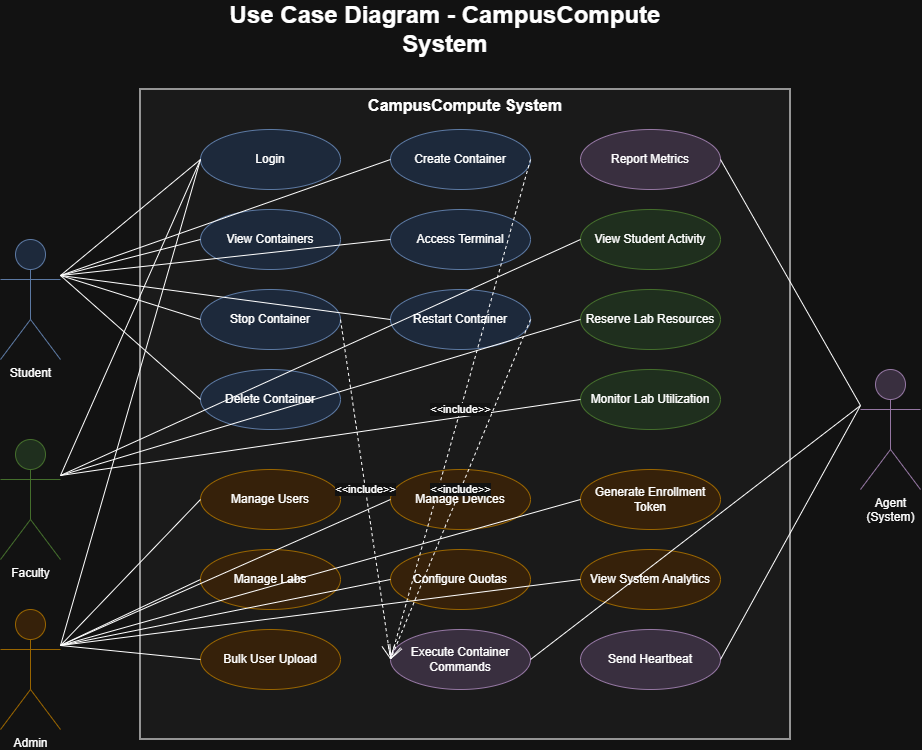
\includegraphics[width=0.85\textwidth]{diagrams/UseCase.png}
\caption{Use Case Diagram - 4 actors, 20 use cases}
\label{fig:usecase}
\end{figure}

Students create and manage containers. Faculty monitor activity. Administrators manage organizations, users, devices. Agents execute commands and report metrics.

\textbf{2.7.2 Class Diagram}

\begin{figure}[ht]
\centering
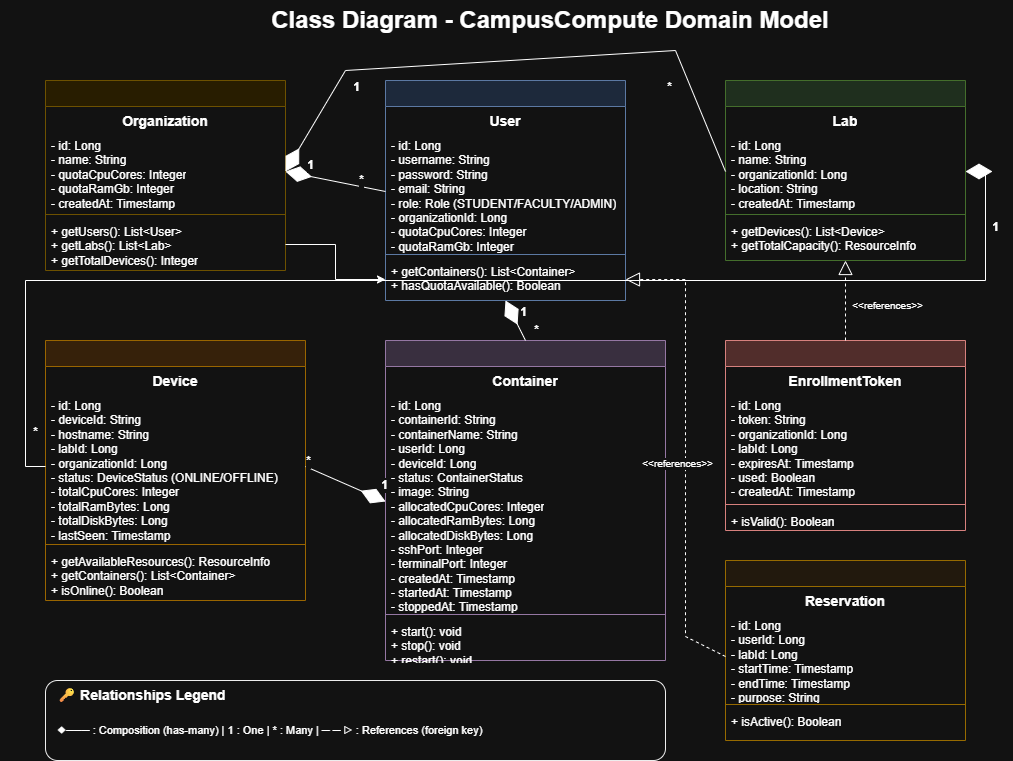
\includegraphics[width=0.85\textwidth]{diagrams/ClassDiagram.png}
\caption{Domain Class Diagram - 7 entities with relationships}
\label{fig:class}
\end{figure}

Organization contains Users and Labs. Labs have Devices which run Containers. Users create Containers.

\textbf{2.7.3 Activity Diagram \& 2.7.4 Sequence Diagram}

These requirements are fulfilled by Collaboration Diagram (Section 2.7.7) showing object interactions and temporal sequence through numbered messages (1-15).

\textbf{2.7.5 Data Flow Diagram (Level 0)}

\begin{figure}[ht]
\centering
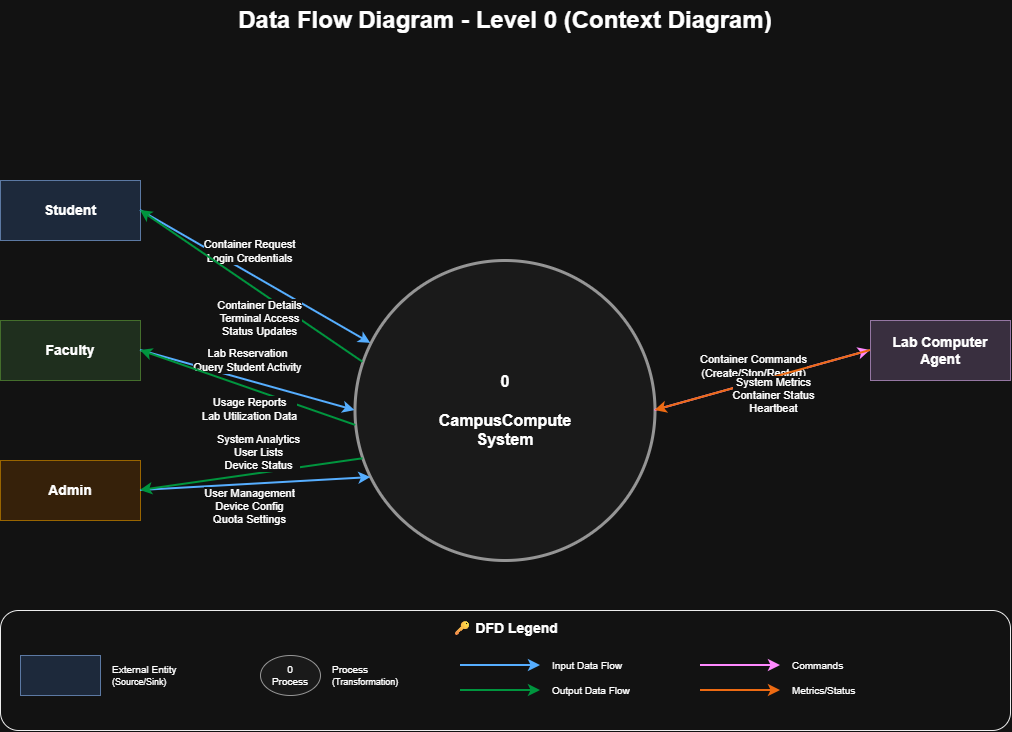
\includegraphics[width=0.85\textwidth]{diagrams/DataFlow.png}
\caption{Context-level DFD - 4 external entities, 8 data flows}
\label{fig:dfd}
\end{figure}

CampusCompute as single process with external entities: Student, Faculty, Admin, Lab Computer Agent.

\textbf{2.7.6 State Diagram}

\textbf{Export needed:} diagrams/2\_container\_lifecycle.drawio to ContainerLifecycle.png

Container lifecycle: 8 states - PENDING, CREATING, RUNNING, STOPPING, STOPPED, RESTARTING, FAILED, DELETED. AWS-style intermediate states ensure UI reflects actual status during transitions.

\textbf{2.7.7 Collaboration Diagram}

\begin{figure}[ht]
\centering
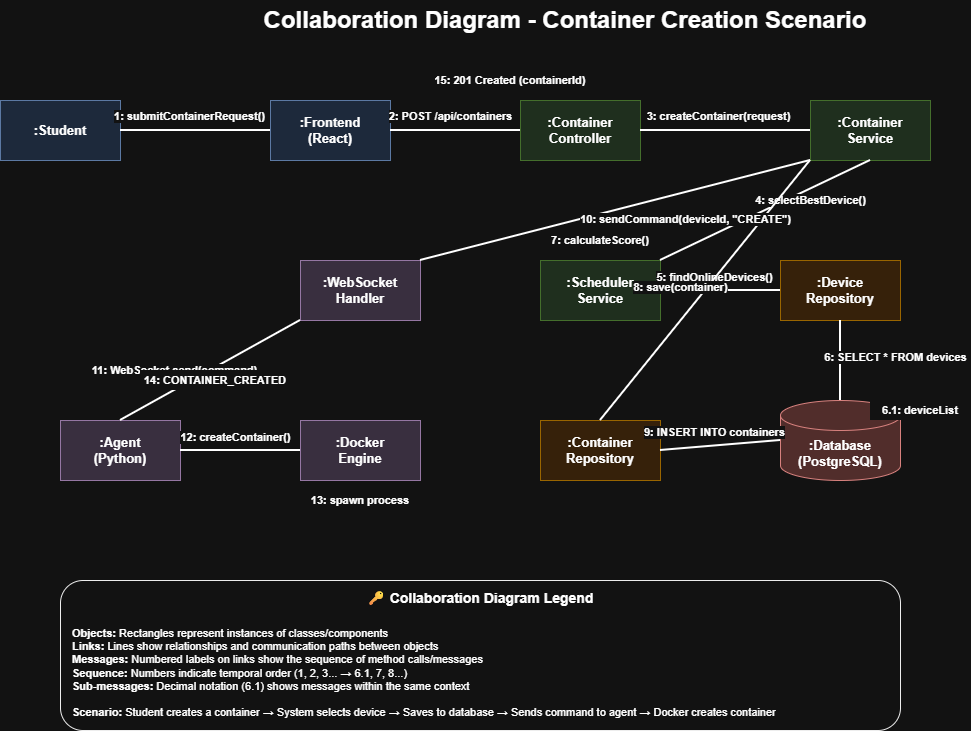
\includegraphics[width=0.85\textwidth]{diagrams/CollaborationDiagram.png}
\caption{Collaboration Diagram - Container creation with 15 messages}
\label{fig:collaboration}
\end{figure}

Complete sequence: (1) Student request, (2-3) Frontend/Controller, (4-7) Scheduler/Database, (8-9) Save container, (10-11) WebSocket command, (12-14) Agent/Docker execution, (15) Confirmation.

\textbf{2.7.8 Deployment Diagram}

\textbf{Export needed:} diagrams/6\_deployment\_architecture.drawio to DeploymentArchitecture.png

Production infrastructure: 3 zones - DMZ (frontend/backend, WebSocket gateway, Redis, monitoring), Internal Network (PostgreSQL primary/replica, backups, NAS), Lab Network (150+ devices, Python Agent, Docker Engine across 15 labs).

\textbf{Cost Analysis:} On-Premise Rs. 8 lakhs (one-time) + Rs. 80k/year vs AWS Rs. 12 lakhs/year. Savings: Rs. 11.2 lakhs/year (93\%).

\textbf{2.7.9 System Architecture (Supplementary)}

\begin{figure}[ht]
\centering
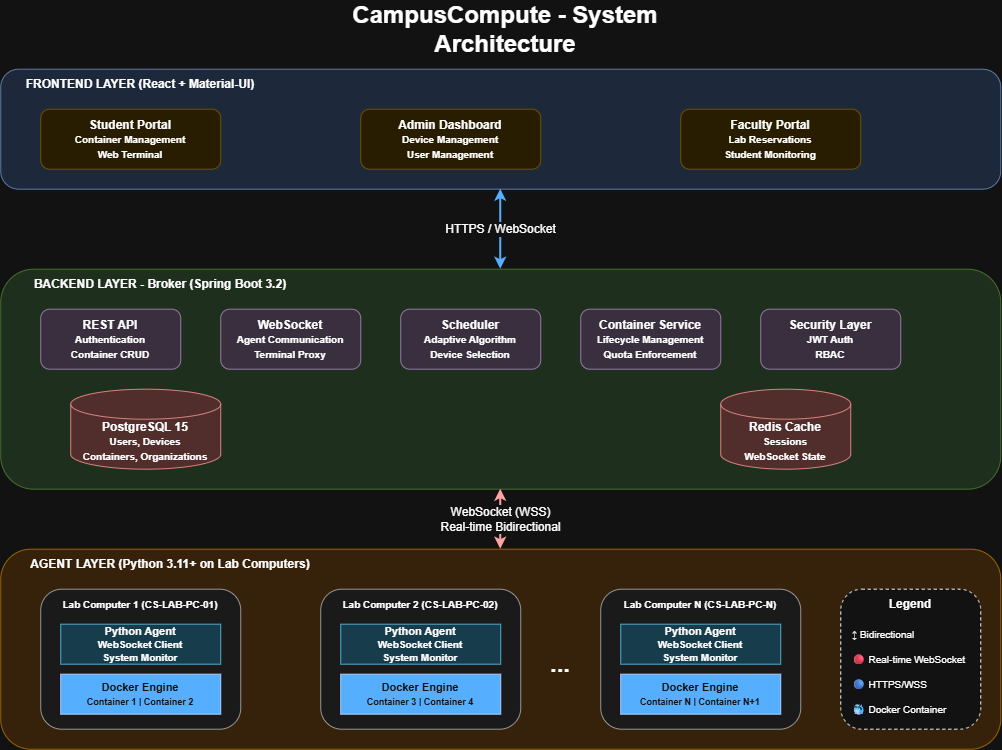
\includegraphics[width=0.85\textwidth]{diagrams/SystemArch.png}
\caption{System Architecture - 3-layer design with WebSocket connections}
\label{fig:systemarch}
\end{figure}

The system follows a 3-tier architecture: Frontend layer (React SPA with terminal emulator), Backend layer (Spring Boot with REST APIs and WebSocket handlers), and Agent layer (Python agents on lab computers with Docker integration). Communication uses HTTP/REST for management operations and WebSocket for real-time terminal access and container commands.

\subsection{Assumption and Dependencies}

\textbf{Assumptions:}

\begin{enumerate}[noitemsep]
    \item Lab computers remain powered on during operating hours (8 AM - 10 PM)
    \item Stable network connectivity between backend and agent machines
    \item Institutional firewall allows WebSocket connections on port 8081
    \item Docker Desktop licenses are available for Windows lab computers
    \item Students have basic Linux command-line knowledge
    \item IT administrators can perform one-time agent installation on lab computers
    \item Backend server has static IP address or DNS hostname
    \item Lab computers are not heavily used for other purposes during idle hours
    \item Students will not attempt container escape or malicious activities
    \item Institutional network has sufficient bandwidth for concurrent terminal sessions
\end{enumerate}

\textbf{Dependencies:}

\textbf{External Dependencies:}
\begin{itemize}[noitemsep]
    \item \textbf{Docker Inc.:} Docker Desktop and Docker Engine availability, licensing terms
    \item \textbf{Docker Hub:} Public image repository accessibility
    \item \textbf{Java/Oracle:} Java 17 runtime availability
    \item \textbf{PostgreSQL:} Database engine stability and updates
    \item \textbf{Python Software Foundation:} Python 3.11+ interpreter
    \item \textbf{Spring Framework:} Spring Boot updates and security patches
\end{itemize}

\textbf{Library Dependencies:}
\begin{itemize}[noitemsep]
    \item Spring Boot Starter Web, WebSocket, Security, Data JPA
    \item React, Material-UI, Redux Toolkit
    \item Python: websockets, docker-py, psutil, pyyaml, pywin32
    \item xterm.js for terminal emulation
    \item PostgreSQL JDBC driver
\end{itemize}

\textbf{Infrastructure Dependencies:}
\begin{itemize}[noitemsep]
    \item Backend server with public IP or campus network accessibility
    \item PostgreSQL database server (can be containerized)
    \item Domain name or IP address for frontend hosting
    \item SSL/TLS certificates for HTTPS in production
\end{itemize}

\textbf{Organizational Dependencies:}
\begin{itemize}[noitemsep]
    \item IT department approval for agent installation
    \item Network administrator cooperation for firewall configuration
    \item User management system integration (optional)
    \item Institutional policies on student resource usage
\end{itemize}

% 3. SYSTEM REQUIREMENTS
\section{SYSTEM REQUIREMENTS}

\subsection{User Interface}

\textbf{3.1.1 Student Portal Interface}

\textit{Components:}
\begin{itemize}[noitemsep]
    \item \textbf{Login Page:} Username/password input, "Remember Me" checkbox, "Forgot Password" link
    \item \textbf{Dashboard:} Container list, resource usage summary, quick create button
    \item \textbf{Create Container Dialog:} Dropdowns for CPU (1-8 cores), RAM (1-16GB), Disk (10-100GB), Image selection (Ubuntu, Alpine, Python, Node.js)
    \item \textbf{Container Card:} Status badge (color-coded), container name, resource allocations, action buttons (Start, Stop, Restart, Delete, Open Terminal)
    \item \textbf{Web Terminal:} Full-screen terminal emulator with xterm.js, resize support, scrollback buffer
\end{itemize}

\textit{Design Requirements:}
\begin{itemize}[noitemsep]
    \item Responsive design (desktop, tablet, mobile)
    \item Material Design principles (Material-UI components)
    \item Loading states with spinners
    \item Error messages with actionable feedback
    \item Success notifications (snackbars)
    \item Real-time status updates via WebSocket
\end{itemize}

\textbf{3.1.2 Admin Dashboard Interface}

\textit{Components:}
\begin{itemize}[noitemsep]
    \item \textbf{Overview Page:} Total devices, active containers, online/offline devices, organization statistics
    \item \textbf{Device Management:} Table with device name, status, CPU/RAM/Disk specs, container count, last seen timestamp, actions (View Details, Remove)
    \item \textbf{User Management:} Table with username, role, organization, active containers, quota usage, actions (Edit, Delete, Reset Password)
    \item \textbf{Lab Management:} List of labs with name, device count, total resources, actions (Edit, Delete)
    \item \textbf{Enrollment Tokens:} Generate token dialog with lab selection, expiration time, view existing tokens
    \item \textbf{Bulk Upload:} CSV file upload for student registration with validation and error reporting
\end{itemize}

\textit{Design Requirements:}
\begin{itemize}[noitemsep]
    \item Data tables with sorting, filtering, pagination
    \item Charts and graphs for analytics (CPU/RAM utilization over time)
    \item Modal dialogs for forms
    \item Confirmation dialogs for destructive actions
    \item Export functionality (CSV, PDF) for reports
\end{itemize}

\textbf{3.1.3 Agent Installer Interface}

\textit{Components:}
\begin{itemize}[noitemsep]
    \item \textbf{Welcome Screen:} Project logo, description, "Next" button
    \item \textbf{Enrollment Token Input:} Text field with validation
    \item \textbf{Installation Progress:} Progress bar (0-100\%), current step description, detailed log output
    \item \textbf{Completion Screen:} Success message, "Finish" button, option to view logs
\end{itemize}

\textit{Design Requirements:}
\begin{itemize}[noitemsep]
    \item Simple wizard-style interface
    \item Clear step-by-step instructions
    \item Error handling with retry options
    \item Windows-native look and feel (tkinter)
\end{itemize}

\subsection{Software Interface}

\textbf{3.2.1 Frontend - Backend Interface}

\textit{Protocol:} HTTP/HTTPS (REST) and WebSocket/WSS

\textit{REST API Endpoints:}
\begin{verbatim}
POST   /api/auth/login           - User authentication
POST   /api/auth/logout          - Logout
GET    /api/containers           - List user containers
POST   /api/containers           - Create container
DELETE /api/containers/{id}      - Delete container
POST   /api/containers/{id}/stop - Stop container
POST   /api/containers/{id}/restart - Restart container
GET    /api/devices              - List devices (admin)
GET    /api/users                - List users (admin)
POST   /api/users                - Create user
POST   /api/labs                 - Create lab
GET    /api/enrollment-tokens    - List tokens
POST   /api/enrollment-tokens/generate - Generate token
\end{verbatim}

\textit{WebSocket Endpoints:}
\begin{verbatim}
/ws/terminal/{containerId}  - Terminal session
/ws/status                  - Real-time status updates
\end{verbatim}

\textit{Data Format:} JSON

\textit{Authentication:} JWT token in Authorization header: "Bearer <token>"

\textit{Error Responses:} Standard HTTP status codes with JSON error objects

\textbf{3.2.2 Backend - Agent Interface}

\textit{Protocol:} WebSocket (bidirectional persistent connection)

\textit{Connection URL:}
\begin{verbatim}
ws://backend:8081/ws/agent?enrollmentToken=xxx&deviceId=yyy
\end{verbatim}

\textit{Message Types (Backend to Agent):}
\begin{verbatim}
CREATE_CONTAINER    - Create new container
STOP_CONTAINER      - Stop running container
RESTART_CONTAINER   - Restart container
DELETE_CONTAINER    - Remove container
PING                - Heartbeat check
\end{verbatim}

\textit{Message Types (Agent to Backend):}
\begin{verbatim}
HEARTBEAT           - Keep-alive signal
CONTAINER_CREATED   - Container successfully created
CONTAINER_STOPPED   - Container stopped
CONTAINER_RESTARTED - Container restarted
CONTAINER_DELETED   - Container deleted
CONTAINER_FAILED    - Operation failed
METRICS             - System resource metrics
\end{verbatim}

\textit{Message Format:}
\begin{verbatim}
{
  "type": "CREATE_CONTAINER",
  "deviceId": 123,
  "organizationId": 1,
  "requestId": "6",
  "timestamp": "2026-10-06T10:30:00Z",
  "payload": {
    "container_name": "container-user-1234",
    "image": "ubuntu:latest",
    "cpu_cores": 2,
    "ram_bytes": 4294967296,
    "disk_bytes": 53687091200
  }
}
\end{verbatim}

\textit{Communication Security:}
\begin{itemize}[noitemsep]
    \item Enrollment token authentication on first connection
    \item Device ID-based authentication on subsequent connections
    \item Message integrity via JSON schema validation
\end{itemize}

\textbf{3.2.3 Agent - Docker Interface}

\textit{Protocol:} Docker Engine API via docker-py (Python SDK)

\textit{Connection Methods:}
\begin{itemize}[noitemsep]
    \item Windows: Named pipe (npipe:////./pipe/docker\_engine)
    \item Linux: Unix socket (unix:///var/run/docker.sock)
\end{itemize}

\textit{Docker SDK Operations:}
\begin{verbatim}
client.containers.run()    - Create and start container
container.stop()           - Stop container
container.restart()        - Restart container
container.remove()         - Delete container
client.containers.list()   - List containers
client.info()              - Get Docker info
\end{verbatim}

\textit{Container Configuration:}
\begin{verbatim}
{
  "image": "ubuntu:latest",
  "name": "container-user-1234",
  "detach": True,
  "tty": True,
  "stdin_open": True,
  "cpu_count": 2,
  "mem_limit": "4g",
  "storage_opt": {"size": "50g"},
  "network_mode": "bridge"
}
\end{verbatim}

\subsection{Database Interface}

\textbf{Database Management System:} PostgreSQL 15+

\textbf{Connection Parameters:}
\begin{verbatim}
Driver: org.postgresql.Driver
URL: jdbc:postgresql://localhost:5432/campuscompute
Username: campuscompute
Password: <configured>
Connection Pool: HikariCP (default in Spring Boot)
Max Pool Size: 20 connections
\end{verbatim}

\textbf{Key Tables:}

\textit{users:}
\begin{verbatim}
- id (BIGSERIAL PRIMARY KEY)
- username (VARCHAR UNIQUE)
- password (VARCHAR, BCrypt hashed)
- email (VARCHAR)
- role (VARCHAR: STUDENT, FACULTY, ADMIN)
- organization_id (BIGINT FK)
- quota_cpu_cores (INT)
- quota_ram_gb (INT)
- first_time_login (BOOLEAN)
\end{verbatim}

\textit{devices:}
\begin{verbatim}
- id (BIGSERIAL PRIMARY KEY)
- device_id (VARCHAR UNIQUE)
- hostname (VARCHAR)
- lab_id (BIGINT FK)
- organization_id (BIGINT FK)
- status (VARCHAR: ONLINE, OFFLINE)
- total_cpu_cores (INT)
- total_ram_bytes (BIGINT)
- total_disk_bytes (BIGINT)
- last_seen (TIMESTAMP)
\end{verbatim}

\textit{containers:}
\begin{verbatim}
- id (BIGSERIAL PRIMARY KEY)
- container_id (VARCHAR UNIQUE)
- container_name (VARCHAR)
- user_id (BIGINT FK)
- device_id (BIGINT FK)
- status (VARCHAR: PENDING, CREATING, RUNNING, STOPPING, 
          STOPPED, RESTARTING, FAILED, DELETED)
- image (VARCHAR)
- allocated_cpu_cores (INT)
- allocated_ram_bytes (BIGINT)
- allocated_disk_bytes (BIGINT)
- created_at (TIMESTAMP)
- started_at (TIMESTAMP)
- stopped_at (TIMESTAMP)
- expires_at (TIMESTAMP)
\end{verbatim}

\textit{organizations:}
\begin{verbatim}
- id (BIGSERIAL PRIMARY KEY)
- name (VARCHAR UNIQUE)
- quota_cpu_cores (INT)
- quota_ram_gb (INT)
- created_at (TIMESTAMP)
\end{verbatim}

\textit{labs:}
\begin{verbatim}
- id (BIGSERIAL PRIMARY KEY)
- name (VARCHAR)
- organization_id (BIGINT FK)
- location (VARCHAR)
- created_at (TIMESTAMP)
\end{verbatim}

\textit{enrollment\_tokens:}
\begin{verbatim}
- id (BIGSERIAL PRIMARY KEY)
- token (VARCHAR UNIQUE)
- organization_id (BIGINT FK)
- lab_id (BIGINT FK)
- expires_at (TIMESTAMP)
- used (BOOLEAN)
- created_at (TIMESTAMP)
\end{verbatim}

\textbf{Indices:}
\begin{verbatim}
CREATE INDEX idx_containers_user ON containers(user_id);
CREATE INDEX idx_containers_device ON containers(device_id);
CREATE INDEX idx_containers_status ON containers(status);
CREATE INDEX idx_devices_status ON devices(status);
CREATE INDEX idx_devices_org ON devices(organization_id);
CREATE INDEX idx_users_org ON users(organization_id);
\end{verbatim}

\textbf{Constraints:}
\begin{verbatim}
ALTER TABLE containers ADD CONSTRAINT containers_status_check
  CHECK (status IN ('PENDING', 'CREATING', 'RUNNING', 'STOPPING', 
                    'STOPPED', 'RESTARTING', 'FAILED', 'DELETED'));

ALTER TABLE devices ADD CONSTRAINT devices_status_check
  CHECK (status IN ('ONLINE', 'OFFLINE'));

ALTER TABLE users ADD CONSTRAINT users_role_check
  CHECK (role IN ('STUDENT', 'FACULTY', 'ADMIN'));
\end{verbatim}

\subsection{Protocols}

\textbf{3.4.1 WebSocket Protocol}

\textit{Standard:} RFC 6455 (WebSocket Protocol)

\textit{Upgrade Request:}
\begin{verbatim}
GET /ws/agent?enrollmentToken=abc123 HTTP/1.1
Host: backend:8081
Upgrade: websocket
Connection: Upgrade
Sec-WebSocket-Key: <base64-encoded-key>
Sec-WebSocket-Version: 13
\end{verbatim}

\textit{Upgrade Response:}
\begin{verbatim}
HTTP/1.1 101 Switching Protocols
Upgrade: websocket
Connection: Upgrade
Sec-WebSocket-Accept: <hash>
\end{verbatim}

\textit{Frame Format:} Binary or text frames with JSON payload

\textit{Ping/Pong:} Heartbeat every 30 seconds

\textit{Closure:} Graceful close with status code 1000 (Normal Closure)

\textbf{3.4.2 HTTP/HTTPS Protocol}

\textit{Standard:} HTTP/1.1 (RFC 7230-7235)

\textit{Methods Used:} GET, POST, PUT, DELETE

\textit{Headers:}
\begin{verbatim}
Authorization: Bearer <JWT-token>
Content-Type: application/json
Accept: application/json
\end{verbatim}

\textit{Status Codes:}
\begin{verbatim}
200 OK                  - Successful request
201 Created             - Resource created
400 Bad Request         - Invalid input
401 Unauthorized        - Authentication required
403 Forbidden           - Insufficient permissions
404 Not Found           - Resource not found
500 Internal Server Error - Server error
\end{verbatim}

\textbf{3.4.3 Security Protocols}

\textit{Authentication:} JWT (JSON Web Tokens) using HMAC-SHA256

\textit{Token Structure:}
\begin{verbatim}
Header: {"alg": "HS256", "typ": "JWT"}
Payload: {"sub": "username", "role": "STUDENT", 
          "organizationId": 1, "exp": 1696598400}
Signature: HMACSHA256(base64(header)+"."+base64(payload), secret)
\end{verbatim}

\textit{Password Hashing:} BCrypt with cost factor 10

\textit{HTTPS:} TLS 1.2 or 1.3 (production deployment)

\textbf{3.4.4 Communication Security}

\textit{Encryption:}
\begin{itemize}[noitemsep]
    \item Production: WSS (WebSocket Secure) with TLS 1.3
    \item Development: WS (unencrypted) for testing
    \item HTTPS for REST APIs in production
\end{itemize}

\textit{Data Transfer Rates:}
\begin{itemize}[noitemsep]
    \item WebSocket messages: <1KB per message
    \item Terminal data: ~10KB/sec (typical), ~100KB/sec (peak)
    \item Metrics data: 2KB per device per minute
\end{itemize}

\textit{Synchronization Mechanisms:}
\begin{itemize}[noitemsep]
    \item Optimistic locking for database updates (version field)
    \item Request ID for correlating commands and responses
    \item Timestamp for message ordering
\end{itemize}

% 4. NON-FUNCTIONAL REQUIREMENTS
\section{NON-FUNCTIONAL REQUIREMENTS}

\subsection{Performance Requirements}

\textbf{4.1.1 Response Time}

\begin{itemize}[noitemsep]
    \item \textbf{API Response Time:}
    \begin{itemize}[noitemsep]
        \item Simple queries (GET user, GET container list): <100ms (95th percentile)
        \item Complex queries (Dashboard statistics): <500ms (95th percentile)
        \item Container creation API call: <200ms (returns PENDING immediately)
    \end{itemize}
    
    \item \textbf{Container Operations:}
    \begin{itemize}[noitemsep]
        \item Container creation (end-to-end): 5-10 seconds (target), 15 seconds (maximum)
        \item Container stop: 2-5 seconds
        \item Container restart: 3-8 seconds
        \item Container deletion: 1-3 seconds
    \end{itemize}
    
    \item \textbf{WebSocket Latency:}
    \begin{itemize}[noitemsep]
        \item Message delivery: <50ms (LAN), <200ms (WAN)
        \item Terminal keystroke latency: <100ms
        \item Status update propagation: <2 seconds
    \end{itemize}
\end{itemize}

\textbf{4.1.2 Throughput}

\begin{itemize}[noitemsep]
    \item \textbf{Concurrent Users:} 500+ simultaneous users
    \item \textbf{API Requests:} 1000 requests/minute (backend)
    \item \textbf{Container Operations:} 50 containers created per minute
    \item \textbf{WebSocket Connections:} 500+ persistent connections
\end{itemize}

\textbf{4.1.3 Scalability}

\begin{itemize}[noitemsep]
    \item \textbf{Devices:} Support 500+ lab computers
    \item \textbf{Containers:} 2000+ concurrent running containers
    \item \textbf{Organizations:} 50+ institutions (multi-tenancy)
    \item \textbf{Database:} 10 million+ records (containers, logs)
\end{itemize}

\textbf{4.1.4 Resource Utilization}

\begin{itemize}[noitemsep]
    \item \textbf{Backend Memory:} <4GB RAM under normal load
    \item \textbf{Backend CPU:} <50\% CPU usage with 100 devices
    \item \textbf{Agent Memory:} <200MB RAM per agent
    \item \textbf{Database:} <8GB RAM for 500 devices
\end{itemize}

\textbf{4.1.5 Capacity}

\begin{itemize}[noitemsep]
    \item \textbf{Concurrent Terminals:} 200+ simultaneous terminal sessions
    \item \textbf{User Accounts:} 10,000+ registered users
    \item \textbf{Historical Data:} 6 months retention for logs and metrics
\end{itemize}

\subsection{Security Requirements}

\textbf{4.2.1 Authentication}

\begin{itemize}[noitemsep]
    \item \textbf{User Authentication:} Username/password with BCrypt hashing (cost factor 10)
    \item \textbf{Session Management:} JWT tokens with 24-hour expiration
    \item \textbf{Agent Authentication:} Enrollment token (one-time use, 24-hour validity) + device ID
    \item \textbf{Token Validation:} HMAC-SHA256 signature verification
    \item \textbf{Password Policy:} Minimum 8 characters, require alphanumeric (future enhancement)
    \item \textbf{Brute Force Protection:} Rate limiting on login endpoint (5 attempts per minute)
\end{itemize}

\textbf{4.2.2 Authorization}

\begin{itemize}[noitemsep]
    \item \textbf{Role-Based Access Control (RBAC):} Three roles (STUDENT, FACULTY, ADMIN)
    \item \textbf{Resource Ownership:} Students can only access their own containers
    \item \textbf{Organization Isolation:} Users can only see resources in their organization
    \item \textbf{Admin Privileges:} Admins can manage all resources in their organization
    \item \textbf{API Authorization:} Every endpoint checks JWT claims and role
\end{itemize}

\textbf{4.2.3 Data Protection}

\begin{itemize}[noitemsep]
    \item \textbf{Encryption in Transit:} HTTPS/WSS with TLS 1.3 (production)
    \item \textbf{Encryption at Rest:} PostgreSQL encryption (optional, via pg\_crypto)
    \item \textbf{Password Storage:} BCrypt hashed passwords, never stored in plaintext
    \item \textbf{Sensitive Data:} Enrollment tokens hashed in logs
    \item \textbf{SQL Injection Prevention:} Parameterized queries (JPA/Hibernate)
    \item \textbf{XSS Prevention:} Input sanitization, Content-Security-Policy header
\end{itemize}

\textbf{4.2.4 Container Security}

\begin{itemize}[noitemsep]
    \item \textbf{Isolation:} Each container runs in isolated namespace
    \item \textbf{No Privileged Access:} Containers run without --privileged flag
    \item \textbf{Resource Limits:} CPU, RAM, disk quotas enforced by Docker
    \item \textbf{Network Isolation:} Bridge network mode, no inter-container communication
    \item \textbf{Image Security:} Use official Docker Hub images, vulnerability scanning (future)
\end{itemize}

\textbf{4.2.5 Privacy}

\begin{itemize}[noitemsep]
    \item \textbf{Data Residency:} All data stored on-premise (no third-party cloud)
    \item \textbf{User Activity:} Logged for audit purposes, not shared externally
    \item \textbf{Container Content:} Not inspected or monitored by system
    \item \textbf{GDPR Compliance:} User data deletion on request (future enhancement)
\end{itemize}

\textbf{4.2.6 Verification and Validation}

\begin{itemize}[noitemsep]
    \item \textbf{Input Validation:} Bean Validation (JSR-380) on all API inputs
    \item \textbf{JWT Verification:} Signature and expiration checks on every request
    \item \textbf{Enrollment Token Verification:} Check expiration, organization, used status
    \item \textbf{Device Heartbeat:} Mark devices OFFLINE if heartbeat missing for 60 seconds
    \item \textbf{Container State Validation:} State machine prevents invalid transitions
\end{itemize}

\subsection{Software Quality Attributes}

\textbf{4.3.1 Adaptability}

The system is designed for easy adaptation to different environments:
\begin{itemize}[noitemsep]
    \item Configuration externalized in application.properties and config.yaml
    \item Support for multiple organizations without code changes
    \item Docker image selection configurable per organization
    \item Quota policies adjustable via admin interface
    \item Database schema supports multi-tenancy
\end{itemize}

\textbf{4.3.2 Availability}

\begin{itemize}[noitemsep]
    \item \textbf{Target Uptime:} 99\%+ (8.76 hours downtime per year)
    \item \textbf{Agent Reconnection:} Automatic reconnection on network failure (5-second retry)
    \item \textbf{Database:} Primary-replica setup for high availability (future)
    \item \textbf{Graceful Degradation:} System continues with reduced capacity if devices go offline
    \item \textbf{Maintenance Window:} Scheduled maintenance during low-usage hours (2-4 AM)
\end{itemize}

\textbf{4.3.3 Correctness}

\begin{itemize}[noitemsep]
    \item \textbf{Functional Correctness:} All features tested against requirements
    \item \textbf{Data Integrity:} Database constraints prevent invalid states
    \item \textbf{Resource Accounting:} Accurate tracking of allocated vs available resources
    \item \textbf{State Consistency:} Container states synchronized between backend and Docker
\end{itemize}

\textbf{4.3.4 Flexibility}

\begin{itemize}[noitemsep]
    \item \textbf{Pluggable Scheduling:} Scoring weights configurable for different algorithms
    \item \textbf{Image Support:} Easy to add new Docker images
    \item \textbf{Authentication:} JWT-based, can integrate with LDAP/OAuth2 (future)
    \item \textbf{Database:} ORM layer allows database migration (PostgreSQL to others)
\end{itemize}

\textbf{4.3.5 Interoperability}

\begin{itemize}[noitemsep]
    \item \textbf{REST API:} Standard HTTP/JSON interface for integration
    \item \textbf{WebSocket:} Standard RFC 6455 protocol
    \item \textbf{Docker:} Compatible with any Docker Engine 24+
    \item \textbf{Browser Compatibility:} Works with all modern browsers
    \item \textbf{Cross-Platform:} Backend runs on Windows/Linux/macOS
\end{itemize}

\textbf{4.3.6 Maintainability}

\begin{itemize}[noitemsep]
    \item \textbf{Code Documentation:} Javadoc for Java, docstrings for Python, JSDoc for JavaScript
    \item \textbf{Logging:} Structured logs (SLF4J in Java, logging in Python)
    \item \textbf{Error Handling:} Centralized exception handlers
    \item \textbf{Modularity:} Layered architecture (Controller, Service, Repository)
    \item \textbf{Version Control:} Git with semantic versioning
\end{itemize}

\textbf{4.3.7 Portability}

\begin{itemize}[noitemsep]
    \item \textbf{Backend:} Java-based, runs on any JVM-compatible OS
    \item \textbf{Agent:} Python-based, supports Windows 10/11 and Linux (Ubuntu 20.04+)
    \item \textbf{Frontend:} Web-based, no installation required
    \item \textbf{Database:} PostgreSQL available on all major platforms
    \item \textbf{Containerization:} Backend can be dockerized for easy deployment
\end{itemize}

\textbf{4.3.8 Reliability}

\begin{itemize}[noitemsep]
    \item \textbf{Mean Time Between Failures (MTBF):} 720 hours (30 days)
    \item \textbf{Mean Time To Recovery (MTTR):} <30 minutes
    \item \textbf{Data Backup:} Daily database backups with 30-day retention
    \item \textbf{Fault Tolerance:} Agent failures don't affect other agents
    \item \textbf{Transaction Management:} Database transactions ensure consistency
\end{itemize}

\textbf{4.3.9 Reusability}

\begin{itemize}[noitemsep]
    \item \textbf{Component Reuse:} Service layer can be used by multiple controllers
    \item \textbf{Code Libraries:} Utility classes for common operations
    \item \textbf{Template Containers:} Pre-configured images for common use cases
    \item \textbf{API:} RESTful design allows third-party integrations
\end{itemize}

\textbf{4.3.10 Robustness}

\begin{itemize}[noitemsep]
    \item \textbf{Error Handling:} Try-catch blocks with meaningful error messages
    \item \textbf{Input Validation:} Reject invalid inputs before processing
    \item \textbf{Resource Limits:} Prevent resource exhaustion (memory, disk, connections)
    \item \textbf{Timeout Handling:} WebSocket and HTTP timeouts prevent hanging
    \item \textbf{Graceful Shutdown:} Clean closure of connections and services
\end{itemize}

\textbf{4.3.11 Testability}

\begin{itemize}[noitemsep]
    \item \textbf{Unit Tests:} JUnit for Java, pytest for Python, Jest for JavaScript
    \item \textbf{Integration Tests:} Spring Boot Test framework
    \item \textbf{API Tests:} Postman collections for endpoint testing
    \item \textbf{Mocking:} Mockito for mocking dependencies
    \item \textbf{Test Coverage:} Target 70\%+ code coverage
\end{itemize}

\textbf{4.3.12 Usability}

\begin{itemize}[noitemsep]
    \item \textbf{Ease of Learning:} Students can create first container in <5 minutes
    \item \textbf{User Documentation:} Student guide, admin guide, installation manual
    \item \textbf{Error Messages:} Clear, actionable error descriptions
    \item \textbf{UI Consistency:} Material Design throughout
    \item \textbf{Accessibility:} Keyboard navigation, screen reader support (WCAG 2.1 Level A)
\end{itemize}

% 5. OTHER REQUIREMENTS
\section{OTHER REQUIREMENTS}

\textbf{5.1 Legal and Licensing}

\begin{itemize}[noitemsep]
    \item System complies with Docker Desktop licensing terms
    \item Open-source dependencies comply with their respective licenses (Apache 2.0, MIT)
    \item No third-party proprietary code used
    \item Institutional approval required before deployment
\end{itemize}

\textbf{5.2 Operational Requirements}

\begin{itemize}[noitemsep]
    \item Backend server must be accessible 24/7
    \item Lab computers should be powered on during usage hours
    \item Regular database backups (daily recommended)
    \item Log rotation to prevent disk space exhaustion
    \item Monitoring and alerting setup (future enhancement)
\end{itemize}

\textbf{5.3 Environmental Requirements}

\begin{itemize}[noitemsep]
    \item Air-conditioned server room for backend server
    \item UPS (Uninterruptible Power Supply) for backend and network equipment
    \item Reliable network infrastructure (switches, routers)
    \item Firewall configuration allowing port 8081 (WebSocket)
\end{itemize}

\textbf{5.4 Disaster Recovery}

\begin{itemize}[noitemsep]
    \item Database backup and restore procedures documented
    \item Configuration files version-controlled in Git
    \item Container data not persisted (ephemeral by design)
    \item Recovery Time Objective (RTO): 4 hours
    \item Recovery Point Objective (RPO): 24 hours (daily backups)
\end{itemize}

\textbf{5.5 Training Requirements}

\begin{itemize}[noitemsep]
    \item Administrator training: 4-hour session covering installation, configuration, troubleshooting
    \item Faculty training: 1-hour session on monitoring and reservations
    \item Student onboarding: 15-minute video tutorial or written guide
    \item Documentation: Admin guide, student guide, API reference
\end{itemize}

\textbf{5.6 Support and Maintenance}

\begin{itemize}[noitemsep]
    \item Bug fixes: Within 48 hours for critical issues
    \item Feature enhancements: Quarterly releases
    \item Security patches: Within 24 hours of discovery
    \item Documentation updates: Concurrent with code changes
\end{itemize}

% APPENDIX A: GLOSSARY
\section*{APPENDIX A: GLOSSARY}
\addcontentsline{toc}{section}{Appendix A: Glossary}

\begin{description}
    \item[Agent:] Software component installed on lab computers that manages Docker containers and communicates with the backend via WebSocket.
    
    \item[API (Application Programming Interface):] Set of HTTP endpoints for programmatic access to system functionality.
    
    \item[Backend:] Central server application (Spring Boot) that coordinates container orchestration, user management, and agent communication.
    
    \item[BCrypt:] Password hashing algorithm used for secure password storage.
    
    \item[Container:] Isolated, lightweight virtualized environment created using Docker technology.
    
    \item[Device:] Lab computer with agent installed that can run containers.
    
    \item[Docker:] Platform for developing, shipping, and running applications in containers.
    
    \item[Enrollment Token:] One-time-use authentication token for registering new agent devices.
    
    \item[Frontend:] Web-based user interface (React application) for students, faculty, and administrators.
    
    \item[Heartbeat:] Periodic signal sent by agent to backend indicating it is still online (30-second interval).
    
    \item[JWT (JSON Web Token):] Compact token format for securely transmitting information between parties.
    
    \item[Lab:] Physical computer lab location containing multiple devices.
    
    \item[Metrics:] System resource measurements (CPU, RAM, disk usage) collected by agents.
    
    \item[Organization:] Top-level entity representing an institution (university, college) in multi-tenant architecture.
    
    \item[PostgreSQL:] Open-source relational database management system used for persistent storage.
    
    \item[Quota:] Resource limit (CPU cores, RAM) assigned to a user or organization.
    
    \item[RBAC (Role-Based Access Control):] Authorization model where permissions are assigned based on user roles.
    
    \item[REST (Representational State Transfer):] Architectural style for designing networked applications using HTTP.
    
    \item[Scheduler:] Component that selects the best device for container allocation using scoring algorithm.
    
    \item[Terminal:] Web-based command-line interface for interacting with containers (xterm.js).
    
    \item[WebSocket:] Protocol providing full-duplex communication channels over TCP connection.
    
    \item[WSS (WebSocket Secure):] Encrypted WebSocket connection using TLS.
\end{description}

% APPENDIX B: ANALYSIS MODEL
\section*{APPENDIX B: ANALYSIS MODEL}
\addcontentsline{toc}{section}{Appendix B: Analysis Model}

\textbf{B.1 Resource Utilization Model}

\textit{Formula for Lab Utilization:}
\begin{verbatim}
Utilization (%) = (Allocated CPU / Total CPU) * 100
\end{verbatim}

\textit{Example:}
\begin{verbatim}
Lab: 50 computers, each with 8 CPU cores = 400 total cores
Current: 30 containers, each using 2 cores = 60 allocated cores
Utilization: (60 / 400) * 100 = 15%
\end{verbatim}

\textbf{B.2 Cost Savings Model}

\textit{AWS Cost for 200 Students:}
\begin{verbatim}
Instance: t3.medium (2 vCPU, 4GB RAM)
Cost: $0.0416/hour = $30/month per instance
200 students * $30 = $6,000/month = $72,000/year
INR equivalent: Rs. 72,000 * 83 = Rs. 59,76,000/year
Rounded: Rs. 60 lakhs/year
\end{verbatim}

\textit{CampusCompute Cost:}
\begin{verbatim}
Backend Server: Rs. 50,000/year (VPS) or Rs. 1,50,000 (on-premise, one-time)
Internet: Rs. 30,000/year
Total: Rs. 80,000/year (cloud) or Rs. 1,80,000 first year (on-premise)
\end{verbatim}

\textit{Savings:}
\begin{verbatim}
AWS: Rs. 60,00,000/year
CampusCompute: Rs. 80,000/year
Savings: Rs. 59,20,000/year (98.7%)
\end{verbatim}

\textbf{B.3 Device Scoring Model}

\textit{Mathematical Formula:}
\begin{verbatim}
Score = Sum(wi * si) where i = 1 to 5

s1 = CPU availability score = (available_cpu / total_cpu) * 100
s2 = RAM availability score = (available_ram / total_ram) * 100
s3 = Disk availability score = (available_disk / total_disk) * 100
s4 = Container load score = (1 - active_containers / max_containers) * 100
s5 = Health score = {100 if healthy, 50 if warning, 0 if error}

Weights: w1=0.30, w2=0.30, w3=0.15, w4=0.15, w5=0.10
Sum(wi) = 1.0 (normalized)
\end{verbatim}

\textbf{B.4 Capacity Planning Model}

\textit{Formula:}
\begin{verbatim}
Max Concurrent Containers = Sum(Device CPU Cores / Avg Container CPU)

Example:
50 devices * 8 cores = 400 total cores
Average container: 2 cores
Max containers: 400 / 2 = 200 containers
Safety margin (80%): 200 * 0.8 = 160 containers
\end{verbatim}

% APPENDIX C: ISSUES LIST
\section*{APPENDIX C: ISSUES LIST}
\addcontentsline{toc}{section}{Appendix C: Issues List}

\textbf{Open Issues (as of October 2026):}

\begin{enumerate}
    \item \textbf{Issue \#1: Terminal Disconnection}
    \begin{itemize}[noitemsep]
        \item \textit{Description:} WebSocket terminal disconnects after 30 minutes of inactivity
        \item \textit{Priority:} Medium
        \item \textit{Status:} Under investigation
        \item \textit{Proposed Solution:} Implement keepalive pings every 60 seconds
    \end{itemize}
    
    \item \textbf{Issue \#2: Docker Installation Requires Restart}
    \begin{itemize}[noitemsep]
        \item \textit{Description:} Agent installer requires system restart after Docker installation
        \item \textit{Priority:} Low
        \item \textit{Status:} By design (Docker requirement)
        \item \textit{Resolution:} Document in user guide, notify user during installation
    \end{itemize}
    
    \item \textbf{Issue \#3: Multi-Device Testing Incomplete}
    \begin{itemize}[noitemsep]
        \item \textit{Description:} System tested on single device, needs validation with 10-20 devices
        \item \textit{Priority:} High
        \item \textit{Status:} Planned for next phase
        \item \textit{Timeline:} 2-3 weeks
    \end{itemize}
    
    \item \textbf{Issue \#4: Linux Agent Installer Not Available}
    \begin{itemize}[noitemsep]
        \item \textit{Description:} Automated installer only for Windows, Linux requires manual setup
        \item \textit{Priority:} Medium
        \item \textit{Status:} Future enhancement
        \item \textit{Proposed Solution:} Create shell script installer for Linux
    \end{itemize}
    
    \item \textbf{Issue \#5: GPU Support Missing}
    \begin{itemize}[noitemsep]
        \item \textit{Description:} Containers cannot access GPU for ML/AI workloads
        \item \textit{Priority:} Low (enhancement)
        \item \textit{Status:} Future roadmap
        \item \textit{Requirements:} Docker with NVIDIA GPU support, CUDA toolkit
    \end{itemize}
\end{enumerate}

\textbf{Resolved Issues:}

\begin{enumerate}
    \item \textbf{Issue \#R1: LazyInitializationException (Resolved Oct 5, 2026)}
    \begin{itemize}[noitemsep]
        \item \textit{Solution:} Added JOIN FETCH queries and Jackson Hibernate6Module
    \end{itemize}
    
    \item \textbf{Issue \#R2: Database Constraint Error on RESTARTING Status (Resolved Oct 5, 2026)}
    \begin{itemize}[noitemsep]
        \item \textit{Solution:} Updated database constraint to include STOPPING, RESTARTING states
    \end{itemize}
    
    \item \textbf{Issue \#R3: Container Stop Shows Error on First Click (Resolved Oct 5, 2026)}
    \begin{itemize}[noitemsep]
        \item \textit{Solution:} Implemented AWS-style intermediate states with delayed refresh
    \end{itemize}
\end{enumerate}

\end{document}
